\documentclass[11pt]{article}

\usepackage[letterpaper,top=1in,bottom=1in,left=1.25in,right=1.25in]{geometry}
\usepackage{setspace}
\usepackage[parfill]{parskip}
\usepackage{hyperref}
\usepackage{enumitem}
\usepackage{tikz,ifthen,xstring,calc,pgfkeys,pgfopts}
\usepackage{tikz-uml}
\usepackage{float}

\tikzumlset{fill class=black!15}

\begin{document}

\begin{figure}

  \begin{center}
    \begin{tikzpicture}

      \umlclass[x=0, y=0, width=15ex]{Engine}{
        unique\_ptr$<$InputHandler$>$ input\_handler \\
        unique\_ptr$<$GameRenderer$>$ renderer 
      }{
        advance( vector$<$unique\_ptr$<$GameComponent$>>$ components )
      }

      \umlclass[x=0, y=-5, width=15ex]{GameComponent}{
      }{
        \umlvirt{update() : void}\\
        \umlvirt{update( InputEvent\& event ) : void}\\
        \umlvirt{accepting\_input() : bool}\\
        \umlvirt{accept\_renderer( GameRenderer\& renderer ) : void}\\
      }

      \umldep{Engine}{GameComponent}

    \end{tikzpicture}
  \end{center}

  \caption{Engine Architecture}

\end{figure}

\end{document}
